%!TEX root = ../dissertation.tex

\chapter{Solution}
\label{chapter:solution}


\section{Overview}
We set out to create an \gls{ide} for \gls{gd} programming that is available as a web application.
To do that, we identified several tasks that the programming environment needs to support in order to be useful for the architect.
It needs to:
(1) let the architect develop programs;
(2) run programs;
(3) display their results;
(4) make it easy to understand programs;
and (5) export results to the most used commercial \gls{cad} applications.

To accomplish these tasks, there are two separate components, as seen in Figure~\ref{fig:archi:sol}: (1) the web application that supports the \gls{ui} for creating programs; and (2) the remote CAD application, that offers an \gls{api} for running programs in \gls{cad} applications.
The first four tasks described above can be handled by the web application alone since there is no need to interact with \gls{cad} applications running in the user's computer.
The fifth task requires both the web application and the remote CAD service.
As also seen in Figure~\ref{fig:archi:sol}, apart from using the web application programming environment \gls{ui}, the architect also needs to install the remote CAD application if and when he wants to export results to \gls{cad} applications.

We made a test implementation of this architecture which we will call Luna Moth from here on.

In the rest of the chapter, we describe these two components and how each of the tasks is implemented in Luna Moth.
Section~\ref{sec:sol:page} describes the web application and its tasks.
Section~\ref{sec:sol:remote} describe the remote CAD service and the export process.

\begin{figure}
  \centering
  
\includegraphics[width=1.0\textwidth]{./images/architecture_overview/architecture_overview}
  \caption{Architecture of the solution.}
  \label{fig:archi:sol}
\end{figure}


\section{Web Application}
\label{sec:sol:page}
To handle the tasks of letting the architect develop programs, running programs, supporting program understanding, and displaying results, the \gls{ui} of the web application has the layout shown in Figure~\ref{fig:page:view}.
Taking up most of the screen space are a text editor (C) and a 3D view (D) that allow the architect to edit a program and view its results.
On top of the text editor and the 3D view are controls for the running process (B), including whether to run automatically and whether to collect data to display traceability.
On the left are hidden panels for actions like selecting a program and exporting to \gls{cad} applications (A).
%{\bf(pictures of panels)}

To help with the implementation, we have used the THREE.js library\footnote{\url{https://threejs.org/} (last accessed on 10/10/2016)} to interact with WebGL\cite{marrin2011webgl} and the Ace Editor library,\footnote{\url{https://ace.c9.io} (last accessed on 10/10/2016)} to provide a syntax highlighted text editor.
%{\bf(React, escodegen, esprima, estraverse, redux)}

%{\bf(describe high-level view of the inner workings of the page)}

\begin{figure}
  \centering
  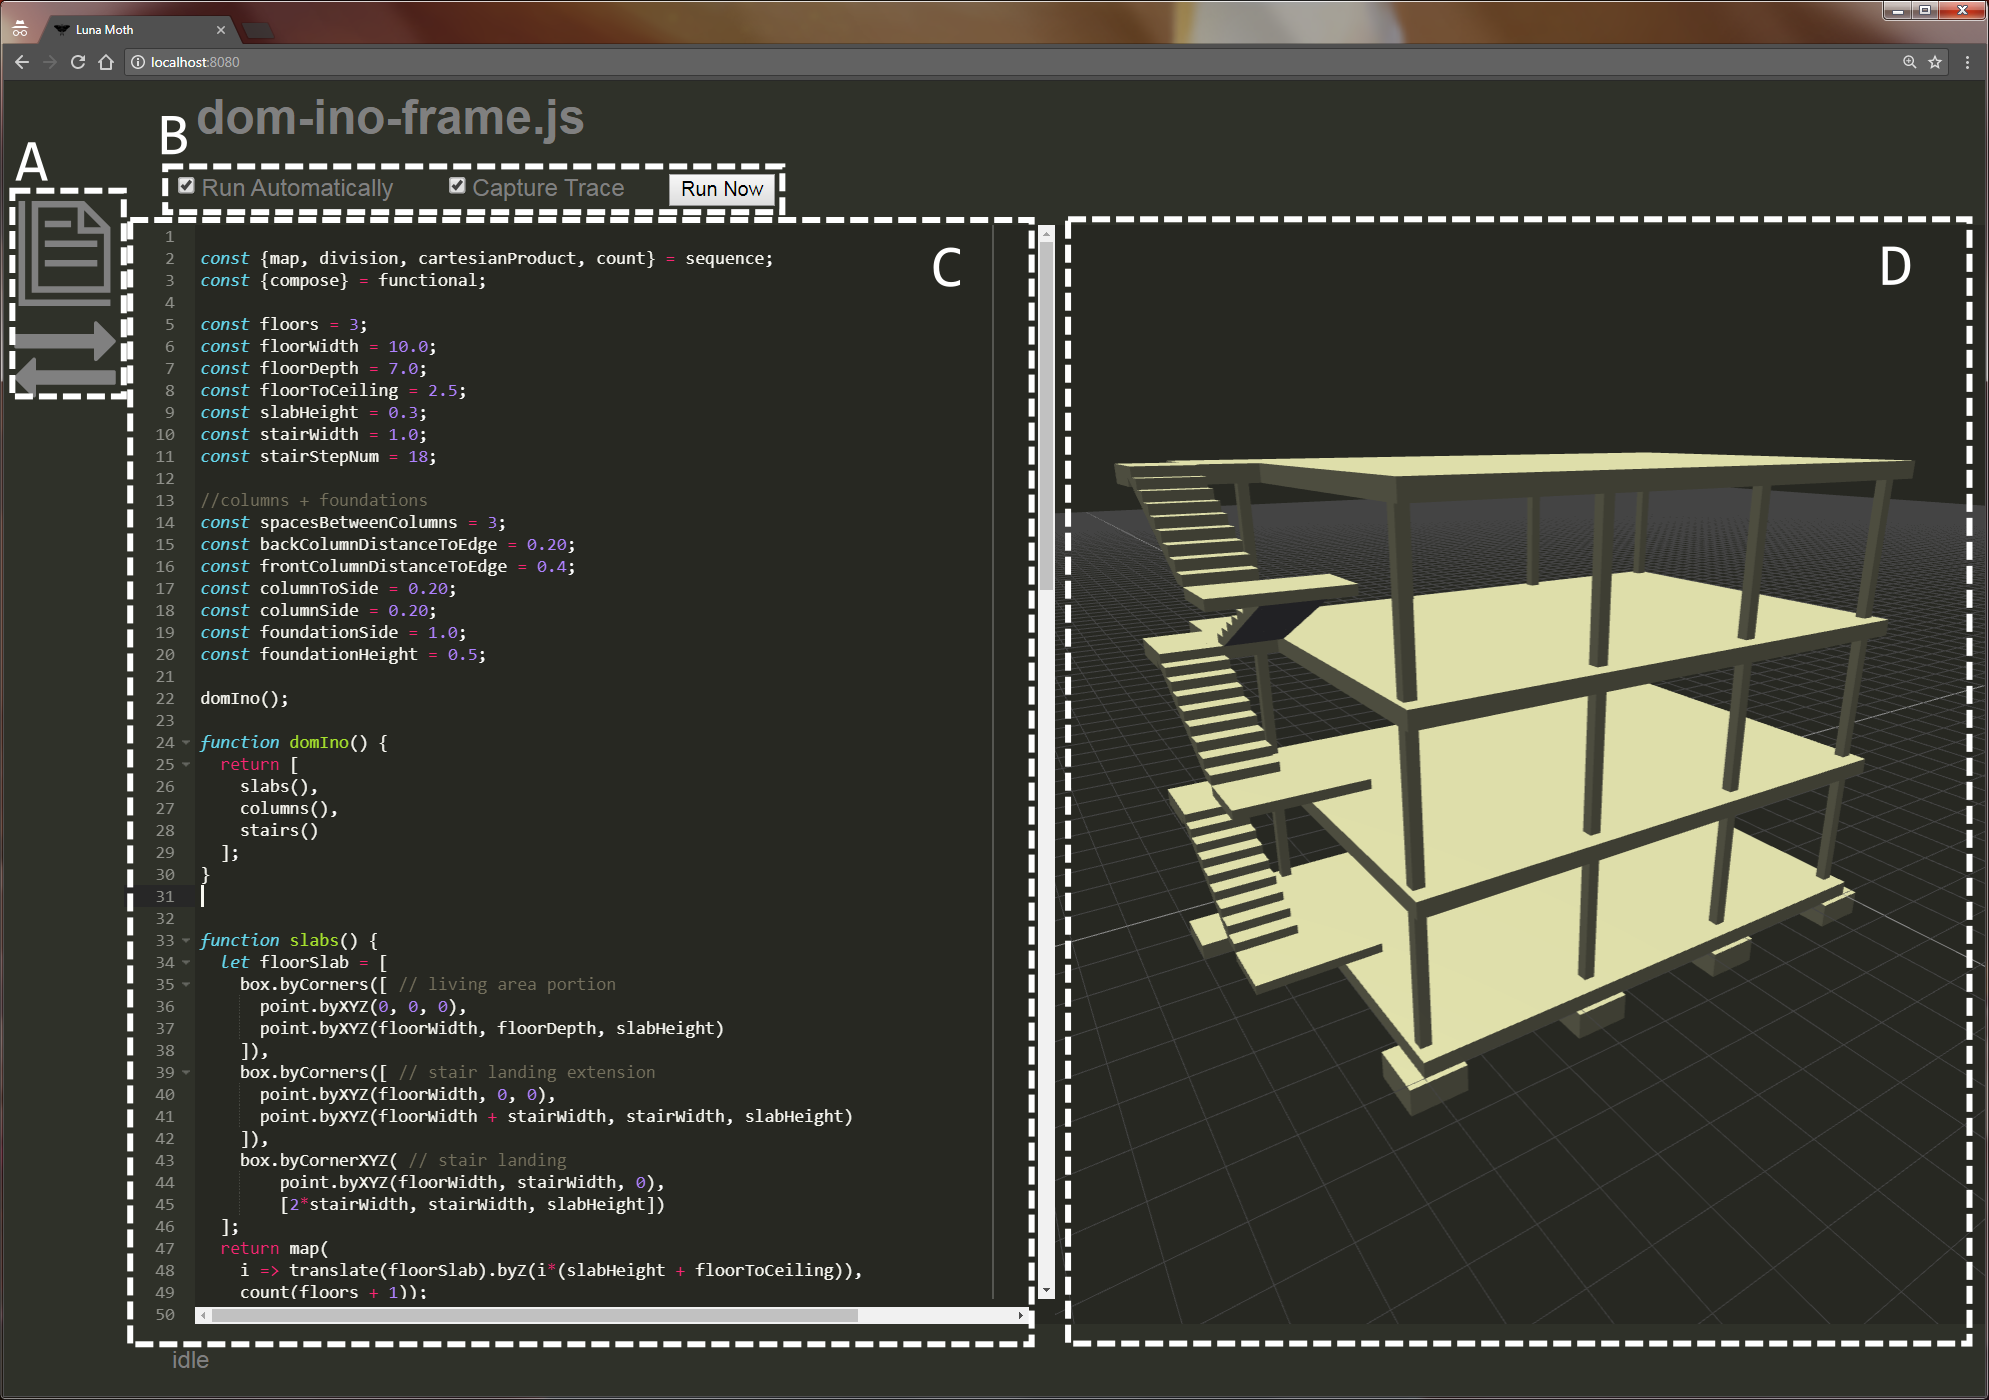
\includegraphics[width=1.0\textwidth]{./images/webpage_view/webpage_view}
  \caption{Layout of the \gls{ui} of the web application.}
  \label{fig:page:view}
\end{figure}


\subsection{Program Comprehension}
In \gls{gd}, the architect interacts with the program that creates the model instead of creating it directly in a \gls{cad} application.
This allows him to automate tasks that normally take too much time and, therefore, also allows him to explore a design space with much more complexity.
However, since he is not directly interacting with the model, he needs to understand the relationship between the program and its results in order to know how to change the program to get the model he wants.
The process of understanding the program and how it relates to its results is called program comprehension\cite{rugaber1995program}.
Luna Moth enables him to do this by providing immediate feedback to changes and by showing traceability.


\subsubsection{Immediate Feedback}
\label{sec:immediate:feedback}
One of the ways to understand the program is to understand the relationship between its inputs and outputs, that is, understanding how each input affects the generated model.
To do this, the architect needs to change the inputs, run the program, see the results, and repeat until he understands the relationship.
This is a tedious process that will bore most architects.
Luna Moth can help them by making this process more immediate.
It must provide quick ways of changing inputs and it must rerun the program when inputs change, so the architect can see the effects of his changes immediately.
This immediacy allows the architect to quickly understand the relationship, which means he is ready to start exploring the design sooner.
Afterwards, he can use the same immediacy to explore the design more efficiently.
To this end, we developed and implemented two different features, namely, the ability to run programs while the architect is writing them, and the ability to efficiently adjust literals.

\paragraph{Adjusting literals}
When a value, such as a number, is typed directly into a program's source code, it is called a literal value, or simply a literal.
When experimenting with a \gls{gd} program, architects find themselves repeatedly adjusting literals that were hardcoded into the program.
This is usually done by retyping parts of the literal's text and, then, re-running the program to see the effect.
Unfortunately, this is annoying and, worse, it makes it difficult to fine-tune the literal.
One possible way to improve this behavior is to automatically re-run the program on every change.
This has the advantage of allowing immediate feedback to changes in literals.

However, editing literals this way often leads to errors, since it is easy to mistype characters.
The architect can increase the literal's value by an order of magnitude if, by mistake, he inserts one character without removing another.
Furthermore, when increasing the literal in steps, different hand movements are required when the increment results in a carry over, e.g. when going from ninety-nine to one hundred, yet again increasing both the likelihood of mistyping and the time it takes to make the changes.
These errors get amplified when the programming environment provides real time feedback and, like so, begins rerunning the program before the error is corrected, leading to annoyance and to reduced \gls{ui} responsiveness.

There are several ways we can extend the user interface to make adjusting literals more user friendly that do not involve manually replacing digits.
They have a simpler mapping to the user's intent.
The following list describes some of them:

\begin{itemize}
  \item {\bf Virtual joystick} Clicking on a literal will display a virtual joystick close to it. When clicked and dragged, it changes the value repeatedly over time, being faster or slower depending on how much the handle is moved from its center.
  \item {\bf Click and drag} Clicking and dragging on a literal will change it according to how much the pointer moved from the starting position.
  \item {\bf Sliders} Clicking on a literal will display a slider. Dragging the slider's handle will change the literal depending on how much the handle is moved from the center of the slider. The slider can have different scales, linear or non-linear, to map the center-handle distance to the amount of change for the literal.
  \item {\bf Keyboard shortcuts} Pressing key combinations while having a literal selected, or the text editor's caret on it, will increment or decrement the literal.
\end{itemize}

Each of the above has its advantages and disadvantages.
The {\it Virtual joystick} and the {\it Sliders}, for example, have the advantage that they are visible to the user and, like so, are easier for him to see and understand.
However, by being visible, they can also block parts of the program that he may want to see.
The {\it Keyboard shortcuts} have the advantage that they do not introduce any visual clutter into the program editor, are more precise, and that they are accessible without getting the hands out of the keyboard.
However, they do require the user to learn their key combinations, which is often avoided by new users.
Lastly, the {\it Click and drag} also has the advantage of not introducing visual clutter into the editor.
Moreover, as with {\it Virtual joystick} and {\it Sliders}, since the interaction is made using the mouse, it is more intuitive for new users.
However, less visual clutter means that the user may not realize that it is possible to adjust the literal.

Taking the advantages and disadvantages of each alternative into account, we decided to implement the {\it Click and drag} way of adjusting literals since it is a good compromise between being easy to use for new users and not introducing visual clutter to the editor.
%Instead of retyping the literal, the user can just ``Click and drag'' on the literal to change its value.
Figure~\ref{fig:lit:adjust} shows an example of its usage.

\paragraph{Implementation}
To implement this behavior, we need to focus on the program editor, as this is where the relevant information is.

The behavior starts when the user presses a mouse button while the pointer is over the text editor.
If it is indeed hovering a numerical literal, we setup an event listener that will update the literal every time the pointer moves until the mouse button is released.

To check that the pointer is over a numerical node, we use the pointer position and the \gls{ast} of the current program.
Since the program will change during the behavior, we keep the path taken through the \gls{ast} to the numerical literal.
We also keep the starting pointer position as a reference for calculating the new literal value when the mouse is moved.

We update the literal by changing the portion of the source code that it represents to the digits representing the new value.
The new value has the same number of fractional digits as the original literal.
To get the new value, we first extract the number of fractional digits and an integer containing the literal's digits and sign (ignoring the decimal point) from the literal's source text.
Afterwards, we add the horizontal distance between the starting point and the current pointer position to the number.
Finally, we convert it back to text and re-add the decimal point.

\begin{figure}
  \centering
  \begin{subfigure}[b]{0.32\linewidth}
    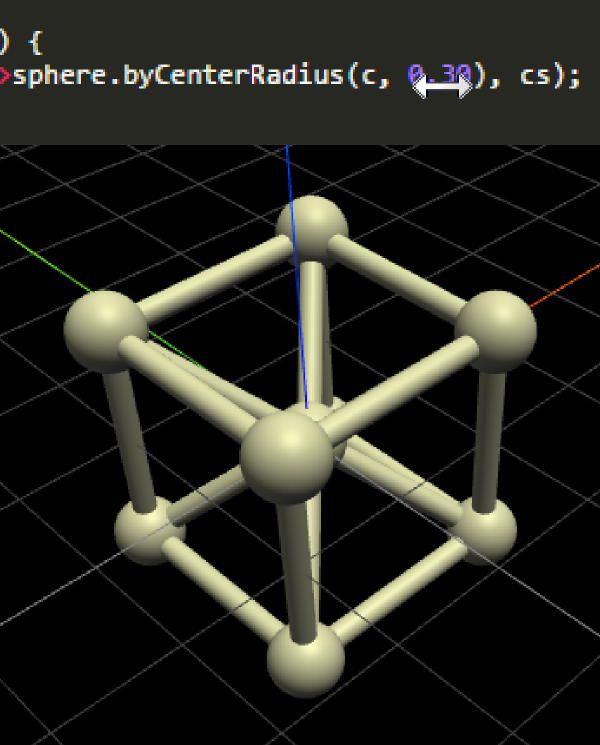
\includegraphics[width=1.0\linewidth]{./images/literal_adjustment/start_crop}
    \caption{Right after clicking.}
  \end{subfigure}
  \begin{subfigure}[b]{0.32\linewidth}
    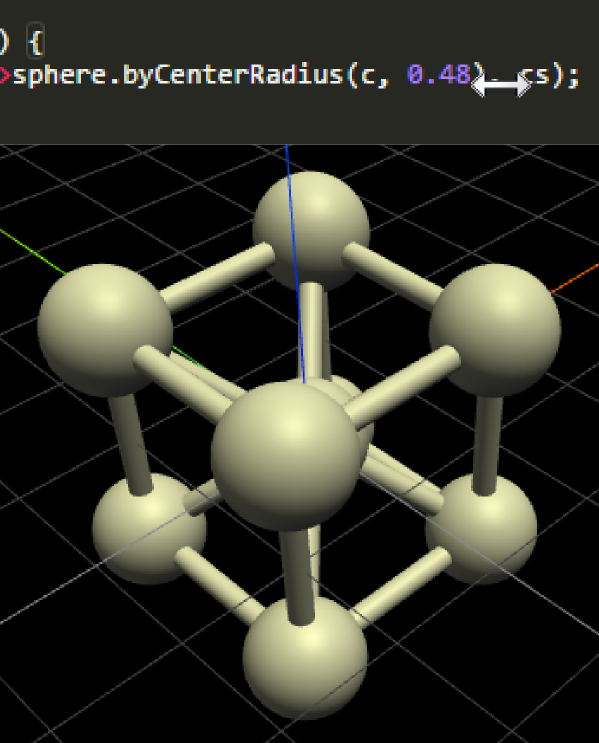
\includegraphics[width=1.0\linewidth]{./images/literal_adjustment/middle_crop}
    \caption{After dragging a little.}
  \end{subfigure}
  \begin{subfigure}[b]{0.32\linewidth}
    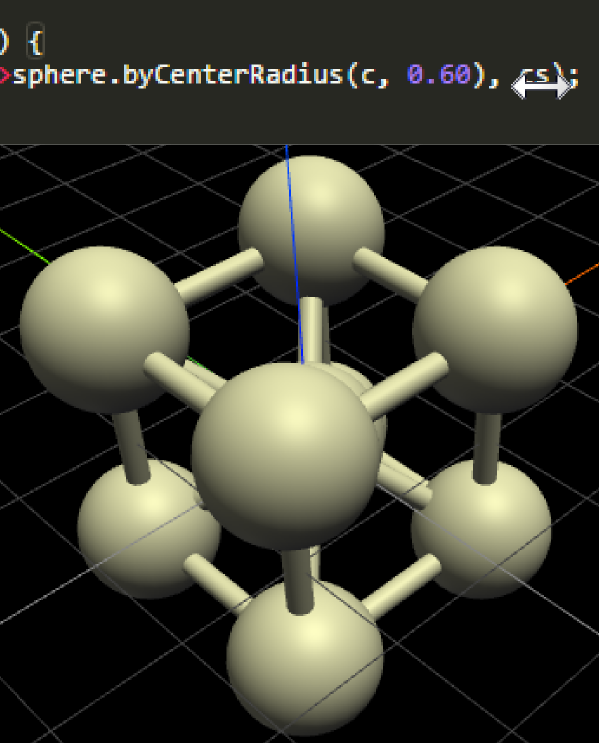
\includegraphics[width=1.0\linewidth]{./images/literal_adjustment/end_crop}
    \caption{After dragging a little more.}
  \end{subfigure}
  \caption{Example of literal adjustment.}
  \label{fig:lit:adjust}
\end{figure}


\subsubsection{Traceability}
\label{sec:traceability}
Reducing the time between making a change and seeing its effect is one way to help the architect to understand a program.

Another way to understand the program is to understand the relationship between parts of the program and parts of the results.
This helps the architect build an understanding of the program from the parts to the whole, and identify both causes of errors and parts that need to be changed to accommodate new design requirements.
This is especially true when he is dealing with programs that generate complex models, where it is much harder to simply look at the program and results and mentally infer the relationship.

If the programming environment takes care of tracking the relation between program and results, the architect only needs to ask for that relation instead of having to track it by himself, freeing his mind to think about the problem.

There are several ways that the environment can use to graphically show the relationship between program and results.
We will describe some of them next:

\begin{itemize}
  \item {\bf Highlighting expressions and results} Every object that is part of the results of a program was created by one expression of that program.
  On the other hand, every expression of the program creates one or more objects of the results.
  The environment can make these relationships visible by changing the appearance of expressions and results when the user points either at an expression or at an object.

  \item {\bf Timetable} As described in Learnable Programming\cite{victor2012learnable}, making things visible makes them more real to the programmer.
  Timetables were proposed as a way to visualize the control flow of programs.
  They act as a map of the program's execution.
  By seeing the control flow, it is easier to see what the program does and it is easier to point at interesting locations.
  By allowing this, timetables provide better navigation inside a program's execution.

  \item {\bf Display data} Also described in Learnable Programming\cite{victor2012learnable}, displaying data would increase the amount of traceability the system provides.
  Apart from being able to see the control flow and the 3D results, seeing the values (e.g. numbers, booleans) that variables and expressions had throughout the program would give the programmer a more complete view of the execution.
\end{itemize}

Each of these alternatives gives the user a different look into what happens as the program runs.
This suggests that they could be used together to increase the environment's traceability.
However, each of them requires additional data collection, which will inevitably increase the running time of programs.
Like so, we have to choose the one that gives the best compromise between being helpful to the programmer and not slowing program execution too much.

When it comes to helping the programmer, the second and third alternatives offer the programmer a better overview of what the program did when it ran, while the first only shows the end-to-end relationship between code and results.

In terms of performance, it is clear that the first alternative will require less data collection since some expressions are guaranteed not to produce 3D results, like arithmetic expressions, while the other two require every step of the program to be recorded.

With these two views in mind, there seems to be a tie between alternatives.
Nonetheless, by taking into account that both {\it Timetable} and {\it Display data} require space in the \gls{ui}, we decided that it was best to implement the {\it Highlighting expressions and results} alternative since its impact on the \gls{ui} is smaller.
Moreover, it can achieve better performance.

\paragraph{Implementation}
The implementation of traceability by highlighting expressions and results requires three things:
(1) collecting traceability data while running a program;
(2) detecting that the user is pointing at either an object from the results or an expression of the program;
and (3) highlighting both the pointed object and the corresponding creator expression, or, in the opposite direction, both the pointed expression and the corresponding created results, as exemplified in Figure~\ref{fig:trace:example}.

To get the traceability data it needs to show the program-results relationship, Luna Moth instruments the program.
We will go into more detail on this matter in Subsection~\ref{sec:run:progs}.

In regard to detecting what the user is pointing at, we follow two approaches depending on the pointer being over the program or over the 3D view.
When the pointer is over the program, we use the program's \gls{ast} annotated with source code locations and the pointer position to find the deepest expression that has recorded traceability data.
When the pointer is over the 3D view, we use ray-casting to detect which of the result objects is below the pointer and closest to the camera.

After detecting that something is being pointed at, Luna Moth needs to highlight it and the corresponding part in the program editor or the 3D view.
To do that, it first uses the traceability data to find the corresponding created objects for an expression, or the first expression that created the pointed object.
Afterwards, it highlights both.
It highlights expressions by changing the program editor's background behind them to a different color.
To highlight 3D objects, it changes their material to a transparent and emissive one, and overlays them on top of the remaining objects.

When working on a larger design, the user may find that the data collection needed to support traceability has a performance impact that he might not want to accept.
In order to solve this problem, we made traceability data collection optional to the user.
This way, he can decide to turn it on when he wants to debug his program or to turn it off when he wants his program to run faster.

\begin{figure}
  \centering
  %
\includegraphics[width=12cm]{./images/traceability_example}
  \begin{subfigure}[b]{1.0\textwidth}
    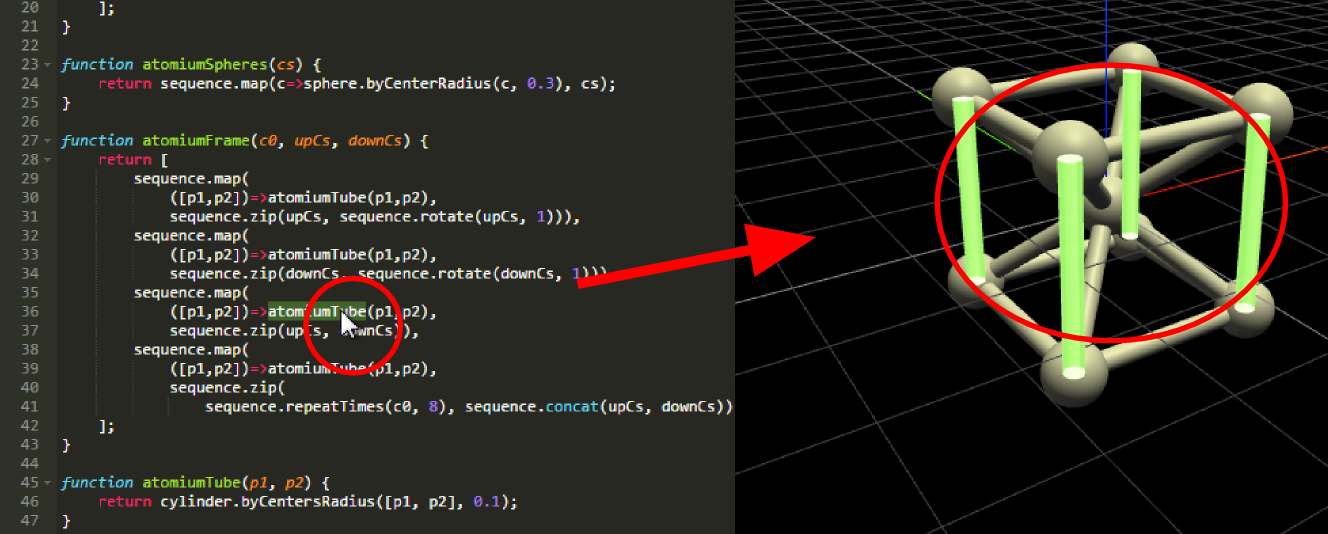
\includegraphics[width=1.0\textwidth]{./images/traceability_example/code_to_results_crop}
    \caption{From code to results.}
    \label{sub:code:to:results}
  \end{subfigure}

  \begin{subfigure}[b]{1.0\textwidth}
    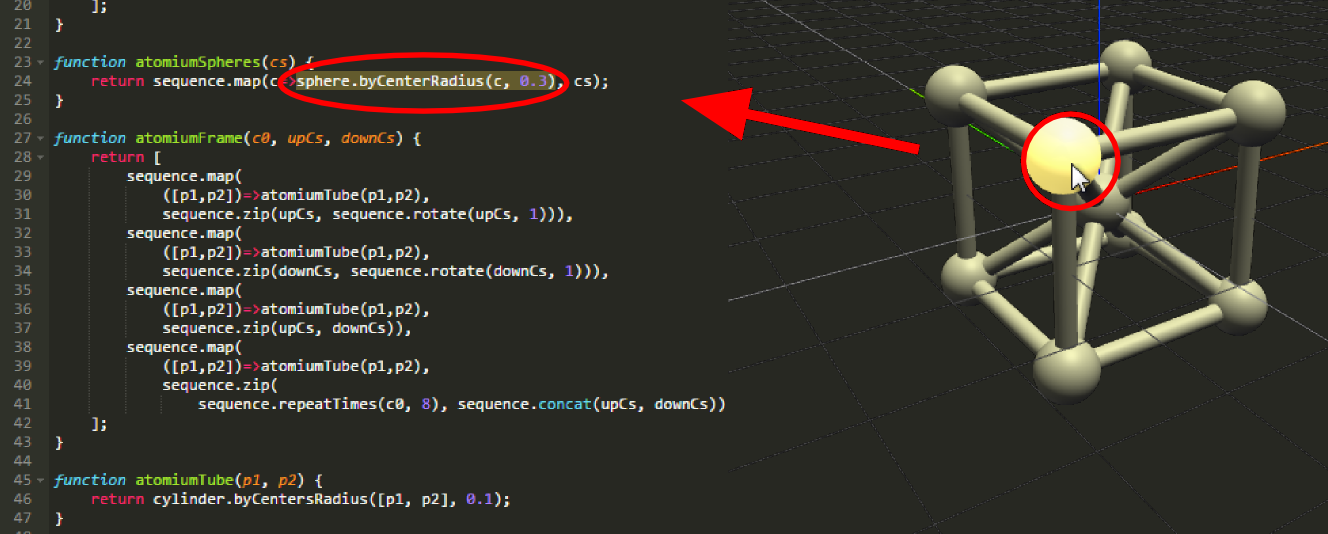
\includegraphics[width=1.0\textwidth]{./images/traceability_example/results_to_code_crop}
    \caption{From results to code.}
    \label{sub:results:to:code}
  \end{subfigure}
  \caption{Two examples of the traceability mechanism. The first from program to results and the second from results to program.}
  \label{fig:trace:example}
\end{figure}


\subsection{Running Programs}
\label{sec:run:progs}
One of the fundamental parts of the programming environment is that it runs programs.
To run programs, the environment needs to support a programming language.
This includes the syntax and semantics of the language and the primitive operations that are available to programs.
After knowing these, the environment must implement a process to run the program and collect results so as to display them later.


\subsubsection{Programming Language}
Everyone can write a text or draw a diagram of what they want the computer to do.
However, if they do not use a concrete and unambiguous language that can be translated automatically by the computer, it will not be possible to get the computer to do what they want.

Luna Moth has to use a programming language that fits the architect's needs.
It can either be an existing language with slight adaptations or a new one specially tailored for their needs.

Still, creating a new programming language is not a realistic option since it would require a great implementation effort to get a working version.
Moreover, since we want programs to run as fast as possible to be able to give architects immediate feedback, further effort would be needed to make it perform fast.

Furthermore, existing programming languages have had time to gather communities that can help the architect when he does not know how to do something or when he is having difficulties correcting a bug.
A new programming language would have a severely limited community.
This suggests that we should use a programming language that already exists.

Architects' experience with programming can vary, however, we can assume that there are more novices than experts.
Like so, Luna Moth needs to have a programming language that is easy to learn and use.
We can consider programming languages that are commonly regarded as good introductory languages such as Python, Racket, and Processing as possible candidates.
Additionally, we can also consider DesignScript, since it was made specifically with computational design in mind\cite{aish2013designscript}, and also JavaScript, since it is readily available in web browsers and was originally made for web designers.

Programming languages have to be translated into the host's language.
For example, to run programs on a typical computer processor, they need to be translated into the {\tt x86} instruction set; to run programs on a virtual machine like the JVM, they need to be translated to its bytecode.
The same is true to run programs on a web browser.
In this case, instead of translating programs into an instruction set or a bytecode, they need to be translated into JavaScript.
Using JavaScript as Luna Moth's language would spare us from a translation step as it is already the target language.
This lead us to choose JavaScript as the programming language supported by the environment.

After having a programming language, there still needs to be a concrete \gls{api} that supports the creation of \gls{gd} programs.
There are things that are essential to support like the creation of geometry, such as coordinates, lines, surfaces, and solids.
Without the \gls{api} supporting these, the architect would need to implement these concepts even before tackling his design problem.
Furthermore, since architects are not trained programmers, it should be easy to create programs that are easy to understand.
Because of that, operations should remain mostly purely functional, i.e. without side-effects.
This way, each operation does only one thing, without modifying the value of any variable, and as a result it is easy to compare its arguments and results.
It behaves more like a mathematical expression.

With a programming language and an \gls{api}, there is still one thing that needs to be decided for Luna Moth to be able to display results to the architect:
how to collect results from programs?

We considered various alternatives:
\begin{itemize}
  \item {\bf Special entry point} Like in OpenJSCAD, we could require that every program must define a function with a special name (e.g. ``main'').
  The environment would then call this function and use its return value as the results of the program.

  \item {\bf Display function} Another way to get results from a program would be giving it access to an output function to the program.
  During its execution, the program would call this function, maybe several times, to produce its output.

  \item {\bf Imperative primitives} A third way to get results would be to add a side-effect to all the 3D object producing functions/primitives.
  Apart from creating the object, they would also add it to the program's results.
  This would be similar to having a display function, as all primitives become specialized display functions.

  \item {\bf Top-level expressions} A fourth way to get results would be to collect them from the expressions at top-level position within the program.
\end{itemize}

Each of this alternatives encourages a slightly different programming approach.
The {\it Imperative primitives} and {\it Display function} alternatives encourage an imperative programming approach, since the programmer must give instructions to create objects or display them.
The {\it Special entry point} and {\it Top-level expressions} alternatives, on the other hand, encourage a functional programming approach since the programmer must specify what objects constitute the results.

We wanted the environment to encourage users to follow a functional programming approach.
Therefore, we did not allow primitives to have side-effects and, like so, we have excluded the alternatives to get results that encouraged imperative programming, namely, {\it Imperative primitives} and {\it Display function}.

Having a {\it Special entry point} is similar to collecting the results of {\it Top-level expressions}, however, it requires the programmer to define a function that returns the results of the program.
When the programmer wants his program to have several results, he will have to aggregate them into a value to provide it as a return value.
This fact lead us to exclude using a {\it Special entry point} as the way Luna Moth uses to collect results.

With all this in mind, we chose to collect the results of {\it Top-level expressions} as the way to collect program results.
Like this, it is easy for the programmer to specify the results of programs since he only has to write the expression at the program's top-level.
Moreover, this approach still encourages him to follow a functional programming approach.
Finally, Listing~\ref{lst:program:example} gives an example of what a program looks like in Luna Moth.

\begin{listing}
\begin{minted}[linenos,frame=lines]{js}
const xyz = point.byXYZ;

function abacus(height, side) {
  return box.byBottomWidthHeightZ(xyz(0,0,0), [side, side], height);
}

function echinus(height, side, neckSide) {
  return coneFrustum.byBottomTopRadiusesHeight(xyz(0,0,0), neckSide/2, side/2, height);
}

function shaft(height, side, neckSide) {
  return coneFrustum.byBottomTopRadiusesHeight(xyz(0,0,0), side/2, neckSide/2, height);
}

function column(height, side, neckSide) {
  return [
    translate(abacus(height*0.05, side)).byZ(height*0.95),
    translate(echinus(height*0.05, side, neckSide)).byZ(height*0.90),
    shaft(height*0.90, side, neckSide)
  ];
}

column(6.00, 0.8, 0.7);
\end{minted}
\caption{An example of a program written in Luna Moth.}
\label{lst:program:example}
\end{listing}


\subsubsection{Running Process}
When Luna Moth runs a program, it needs to do two things: (1) collect the results of the program; and (2) collect traceability data.
It does these two by instrumenting the program with additional calls to special functions that record the desired information, then running the program, and afterwards collecting the results from the instrumentation.
As stated in \ref{sec:traceability}, the collection of traceability data is optional since it adds some overhead to program execution, which may be undesired when programs start to take too much time to run.

To be able to perform the instrumentation, Luna Moth parses the program using Esprima, a JavaScript parser,\footnote{\url{https://github.com/jquery/esprima} (last accessed on 10/10/2016)} to get its \gls{ast}.%
\footnote{The \gls{ast} conforms to a community standard. It can be found at \url{https://github.com/estree/estree} (last accessed on 10/10/2016).}

Afterwards, the \gls{ast} is transformed by adding a recording call to (1) all top-level expression statements and (2) all function call expressions.
Figure~\ref{fig:instrument:example} exemplifies the transformation.
To let the recording functions know what top-level expression or function call is producing a result, we also provide them with identifiers for those expressions.

After this step, Luna Moth creates a new function with the instrumented program as its body.
The primitives and recording functions are provided as parameters to this new function.

Finally, the newly created function is called and, afterwards, the recorded information is made available to the rest of the system.

\begin{figure}
  \centering
\begin{minipage}[c]{0.3\linewidth}
  \center{Before}
  \begin{minted}[frame=lines]{js}
let s = sphere.byRadius(5);
s;
  \end{minted}
\end{minipage}%
\hspace{0.045\linewidth}%
\begin{minipage}[c]{0.3\linewidth}
  \includegraphics[width=1.0\linewidth]{./images/prog_ast/prog_ast}
\end{minipage}%
\hspace{0.045\linewidth}%
\begin{minipage}[c]{0.3\linewidth}
  \center{After}
  \begin{minted}[frame=lines]{js}
let s = recordCallResult(
   sphere.byRadius(5),
   /*function call ID*/);
recordTopLevelResult(
   s,
   /*top-level expr ID*/);
  \end{minted}
\end{minipage}
  \caption[A program before and after the transformation.]{A program before and after the transformation. Its \gls{ast} is also shown, with the function call highlighted in blue and the top-level expression highlighted in red.}
  \label{fig:instrument:example}
\end{figure}


\subsubsection{Displaying Results}
After running the program, Luna Moth needs to display a rendering of the results to the architect.
Displaying results is deeply tied to what programs can produce since their results must be converted to a representation that can be rendered.
The \gls{api} used by those programs is what determines which results can be produced.
Luna Moth uses THREE.js for 3D rendering.
By using THREE.js, the implementation effort is reduced since, on top of implementing rendering, THREE.js also implements several geometric primitives useful for \gls{gd} and implements ray-casting.
However, since Luna Moth provides a functional \gls{api} and THREE.js's \gls{api} is imperative, it needs to cover the differences between these two \glspl{api}.

The main difference between them lies in how they support reuse.
THREE.js's \gls{api} makes it difficult to reuse objects since it only allows scenegraph objects to have one parent.
If the programmer wants to reuse one object, he has to clone it.
Luna Moth's \gls{api}, on the other hand, does not impose this rule.
To cover the difference, we use two steps:
(1) we run the program using the functional \gls{api}, creating intermediary results;
and (2) we convert those results to objects from THREE.js's \gls{api}, cloning them when necessary.

Consider the program in Listing~\ref{lst:display:example}, which creates spheres on the vertices of a cube of width {\tt w}.
Figure~\ref{fig:display:results} shows the overall process from having a program to displaying its results.
After running the program, results are in the form shown in \ref{sub:fig:prog:res}, where the variable {\tt g} holds several translations ({\tt +xyz}) of the same sphere ({\tt sph}).
The next stage converts these results to a THREE.js scenegraph, creating a mesh for {\tt sph}, then copying it for each translation, resulting in the ``{\tt sph~:~Mesh}'' objects seen in \ref{sub:fig:three:res}. Afterwards, these object are grouped as children of the ``{\tt g : Object3D}'' object.
After having results converted to THREE.js objects, Luna Moth issues their rendering repeatably as the architect interacts with the 3D view.

Luna Moth also keeps record of the correspondence between intermediary results and THREE.js objects.
Together with the correspondence between program nodes and intermediary results, this information is used to enable support for showing traceability.


\begin{listing}
\begin{minted}[linenos,frame=lines]{js}
function sphereCube(w, sphR) {
  let sph = sphere.byRadius(sphR);
  return [
    translate(sph).byXYZ(0, 0, 0),
    translate(sph).byXYZ(w, 0, 0),
    translate(sph).byXYZ(w, w, 0),
    translate(sph).byXYZ(0, w, 0),
    translate(sph).byXYZ(0, 0, w),
    translate(sph).byXYZ(w, 0, w),
    translate(sph).byXYZ(w, w, w),
    translate(sph).byXYZ(0, w, w)
  ];
}

let g = sphereCube(10, 1);
g;
\end{minted}
\caption{A program creates spheres on the vertices of a cube.}
\label{lst:display:example}
\end{listing}


\begin{figure}
  \centering
  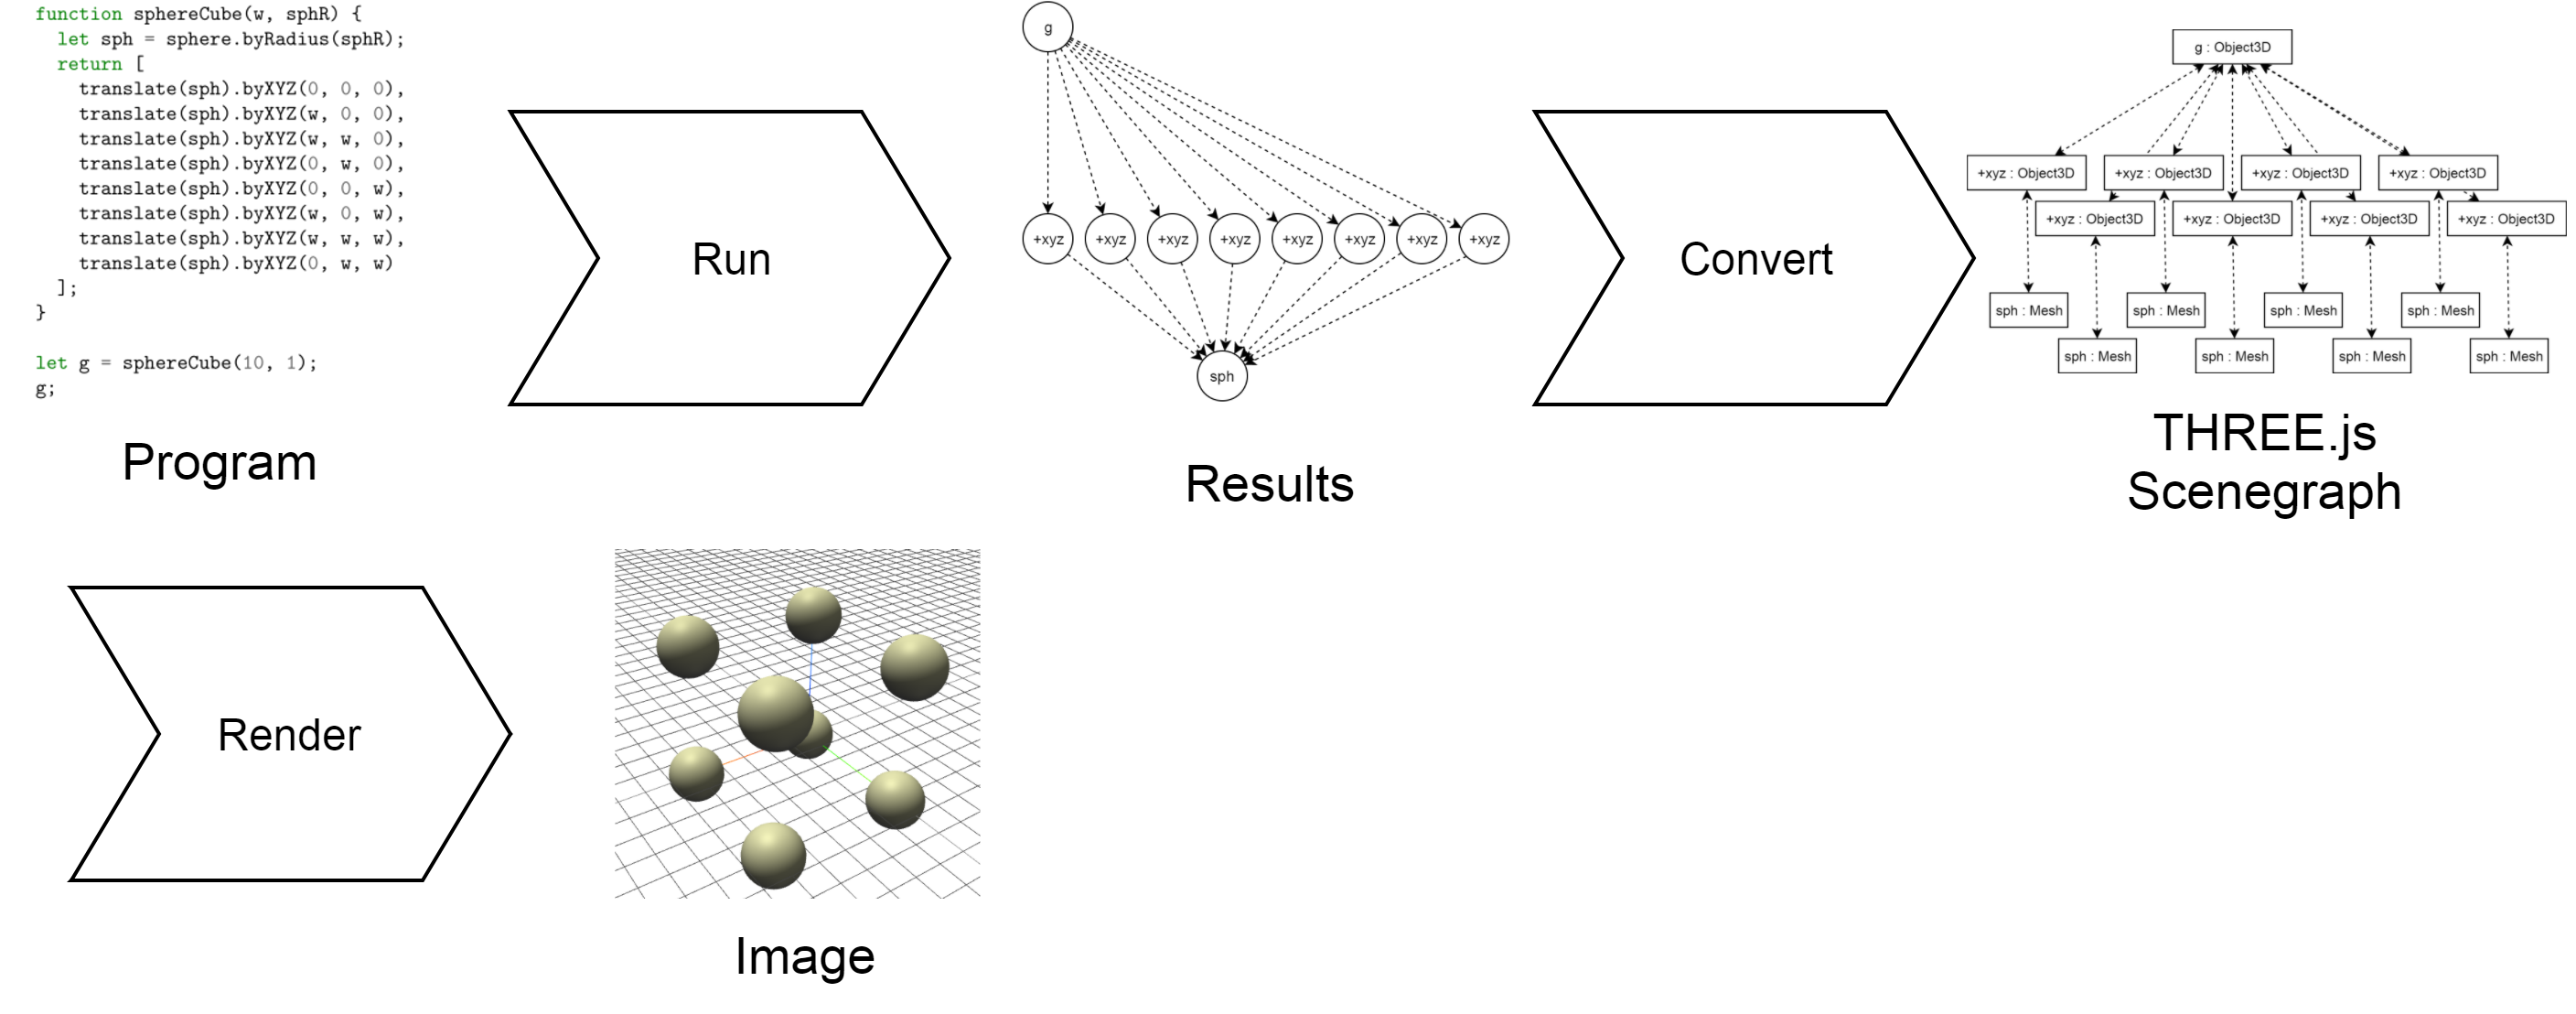
\includegraphics[width=1.0\textwidth]{./images/display_results/display_results}
  \caption{The process used to display results.}
  \label{fig:display:results}
\end{figure}

\begin{figure}
  \centering
  \begin{subfigure}[b]{0.49\textwidth}
    \includegraphics[width=1.0\textwidth]{./images/display_results/results}
    \caption{Program results}
    \label{sub:fig:prog:res}
  \end{subfigure}
  \begin{subfigure}[b]{0.49\textwidth}
    \includegraphics[width=1.0\textwidth]{./images/display_results/three}
    \caption{THREE scenegraph}
    \label{sub:fig:three:res}
  \end{subfigure}
  \caption[Comparison of program results structure and THREE.js scenegraph.]{Comparison of program results structure and THREE.js scenegraph. Arrows indicate that the object at their root has a reference to the object they point to.}
  \label{fig:results:vs:three}
\end{figure}


\section{Remote CAD Service / Exporting to CAD}
\label{sec:sol:remote}
The last task that Luna Moth needs to support is exporting to the most used commercial \gls{cad} applications.

As opposed to the other tasks, exporting to a \gls{cad} application requires the web page to communicate with other applications.
To do so, it must locate the \gls{cad} application and connect to it.
In addition, there must be a well-defined interface of operations that can be performed in the \gls{cad}, which needs to cover the operations that can be performed in programs, as well as operations for managing the \gls{cad}'s document.

To make communication possible, Luna Moth includes an application, the \textit{remote CAD app}, that the architect must install and run in his computer when he wants to export results.
This application serves as a bridge between \gls{cad} applications installed in the computer and the environment running in the web page.
After being started, the application detects which \gls{cad} applications are installed in the computer and connects to the \textit{environment directory} so it can be discovered by the web application.
When the architect needs to export a program to his \gls{cad} application, the environment connects to the application in his computer through the \textit{environment directory} and starts to send requests to it, in order to create shapes in the \gls{cad} application.
The architecture for this part of Luna Moth is illustrated in Figure~\ref{fig:remote:cad:archi}.

Figure~\ref{fig:remote:cad:example} shows an example of the export to \gls{cad} functionality.
The architect has created a program using Luna Moth.
After selecting AutoCAD and SketchUp as export destinations, he starts the export process and, afterwards, the model resulting from running the program is available in both \gls{cad} applications.

Note that it is only needed to install the \textit{remote CAD app} if and when the architect wants to get the program's results on a \gls{cad} application.
Furthermore, the application only needs to be installed in the computer that actually has the \gls{cad} application installed.


\subsection{Implementation}
We implemented the \textit{remote CAD app} as a small Racket server.
It expects to receive HTTP requests for operations like adding shapes to the currently selected \gls{cad} applications or deleting all shapes they may have.
It also expects requests for specifying what \gls{cad} applications are selected.

Apart from the connection between the remote CAD application and the web application, there also needs to be a connection between the remote CAD application and the \gls{cad} applications themselves.
Different \glspl{cad} have different \glspl{api} so the application needs to know how to interact with each one.

Instead of implementing the connection with \gls{cad} applications, the \textit{remote CAD app} uses Rosetta as an intermediate.
This way, it only has to cover the semantic differences between Rosetta's \gls{api} and the remote CAD service's \gls{api}.

In reality, when the architect wants to export to \gls{cad}, it is likely that he is using the web environment in the same computer where he has the \gls{cad} application installed.
Like so, the web page, the remote CAD application and the \gls{cad} applications are running in the same computer.
With this in mind, we chose to temporarily host the web application containing the \gls{ide} in the \textit{remote CAD app}'s server.
Using this setup, it is easier to test the communication between the page and the application.
Moreover, this setup also avoids dealing with cross-origin restrictions imposed by web browsers for \gls{ajax} requests.

\begin{figure}
  \centering
  \includegraphics[width=1.0\textwidth]{./images/export_archi_over/export_archi_over}
  \caption{Illustration of the remote CAD service's architecture.}
  \label{fig:remote:cad:archi}
\end{figure}


\begin{figure}
  \centering
  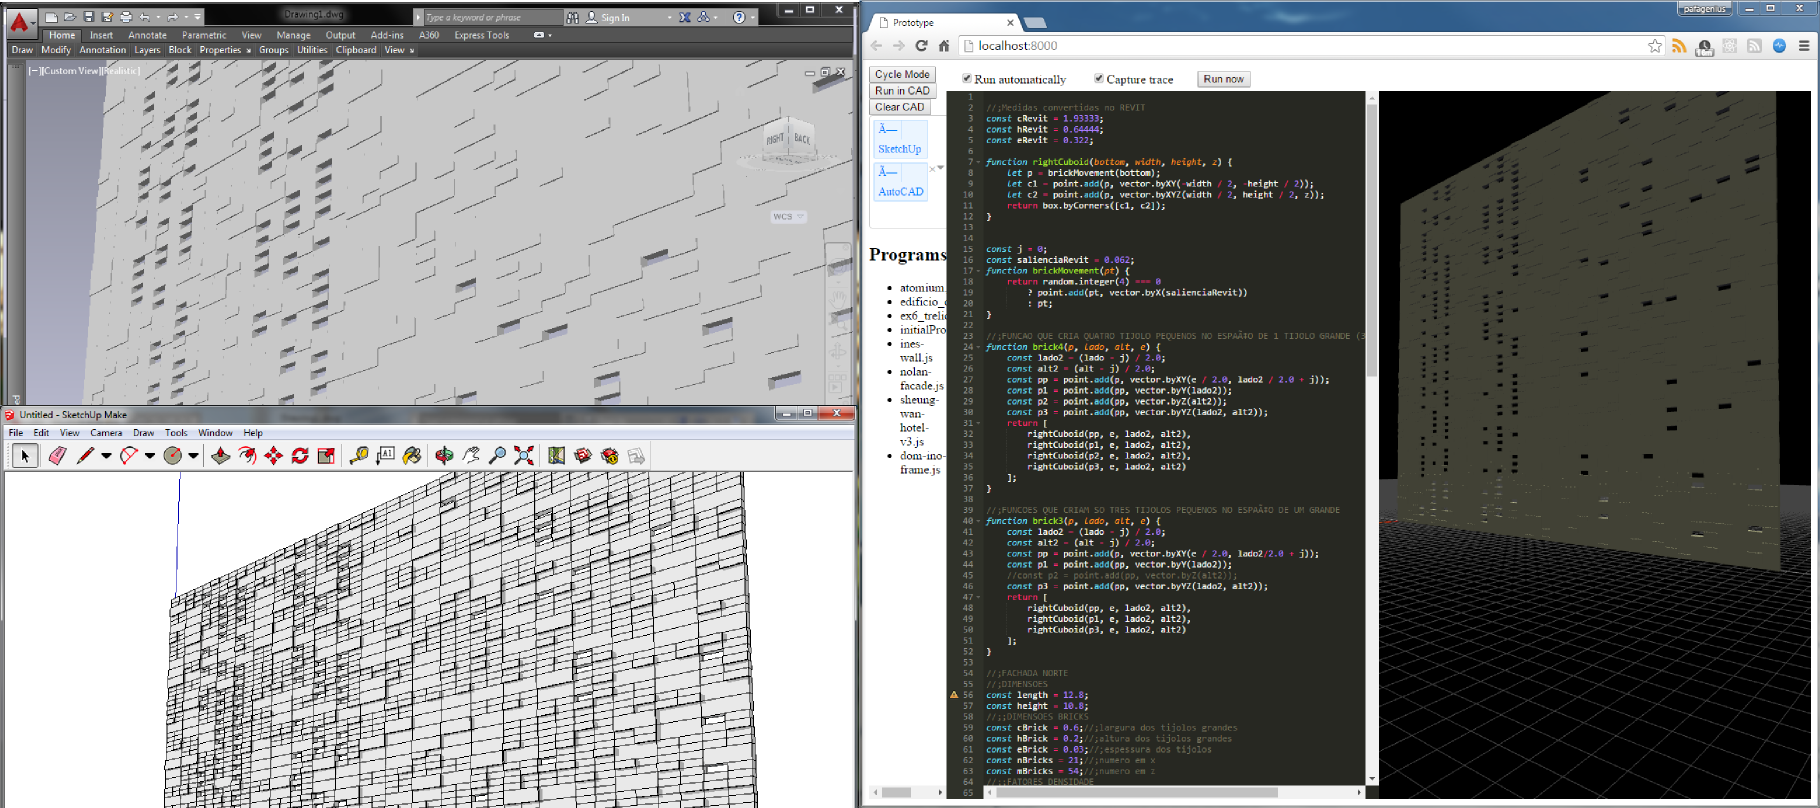
\includegraphics[width=1.0\textwidth]{./images/remote_cad_example/remote_cad_example}
  \caption[An example of the remote CAD service.]{An example of the remote CAD service. The results of the program have been passed to both AutoCAD and SketchUp.}
  \label{fig:remote:cad:example}
\end{figure}


%Design principles / Guiding ideas
%- Ideas based on observations from related work?

%Architecture - Show the overview of the architecture
%- Web page + remote CAD service

%Web page
%- Architecture
%- Page Layout
%- Features / What needs to be done by the IDE?
%   - Discussion + Decision
%   - Implementation
%- Problems
%   - Adjusting source code values
%   - Instrumenting and running programs
%     - Getting results / What is a program?
%     - Providing primitives/predefined bindings
%     - Handling traceability
%   - (Running programs blocks the UI)
%   - Displaying 3D results

%Remote CAD service
%- Architecture
%- Problems
%   - Supporting multiple CADs
%   - Defining the API

%Problem: Handling CAD communication
